\chapter{Introduction}
\label{cpt:format}

% small blurb summary

\section{APT Background}

The Advanced Particle-astrophysics telescope is designed to be a successor to the Fermi Gamma-ray Space Telescope, which is nearing its 12th year in operation of a planned 10-year mission. The main objectives of the APT include studying high-energy transient phenomena such as supernovae or gamma-ray bursts (GRBs), continuing the search for dark matter, and conducting broader surveys of the sky in gamma rays. The APT would improve telescope sensitivity while maintaining a similar budget to the Fermi mission, allowing for a more extensive search for dark matter and an increased ability to detect high-energy transients.

\section{APT Design}

The APT is designed to be used in the mid-keV to low TeV energy range, which is a significant improvement on Fermi's detecting range. The final telescope will consist of 20 repeated layers of detecting material, spaced 15 cm apart, in a cube 3 meters tall and 2.5 meters on each side. The middle section of each layer - the calorimeter - records the energy of each particle that interacts with it, and the WLS fibers on the top and bottom of each layer record the corresponding position of each interaction. From these detected interactions, we are able to reconstruct the initial direction of the photon source using software.

\begin{figure}
    \centering
    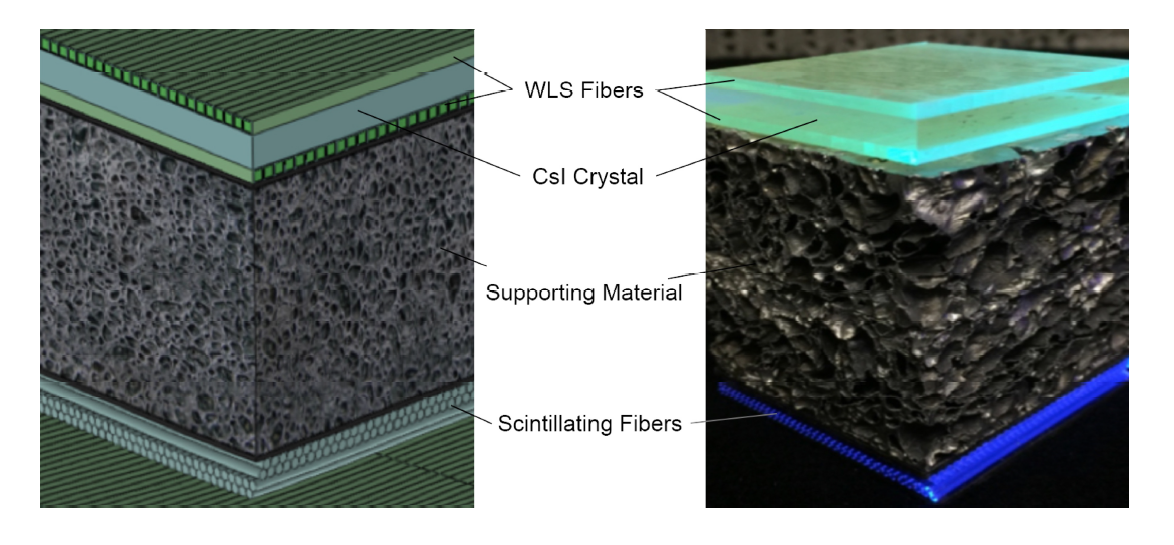
\includegraphics[width=0.7\textwidth]{APT_layers.png}
    \caption{One layer of the APT, shown as a computer model on the left and as a real-world prototype on the right, with aluminum used for the support structure. The Cesium Iodide (CsI) detects photon energy while the WLS fibers detect photon position. The scintillating fibers detect the position of any matter particles that enter the detector. Each subsequent layer would have the same structure as the one shown. \cite{APTmemo}}
    \label{fig:APT_layer}
\end{figure}

\section{APT Software}
The APT achieves such a broad energy range by using two different software methods for reconstructing the trajectories of incoming photons, one for each of the two dominant gamma-ray interactions in this energy range. Below approximately 30 MeV, the dominant interaction is called Compton scattering, a process by which a photon transfers some of its momentum to an electron, changing its resulting wavelength and trajectory. In the mid-MeV to GeV range, photons most commonly undergo a process called pair production upon entering the detector. As this research focuses on reconstructing Compton scatters, a thorough discussion of pair production is outside the scope of this paper, but more information can be found in almost any particle physics textbook or online.

\section{Related Work}
- Boggs & Jean
        - focused more on the physics than the CS
        - Gives us a basic algorithm to improve upon
- Zoglauer's Megalib
- terrestrial gamma-ray imaging

\section{Gamma-ray Bursts}
- extremely bright bursts of gamma-rays from point sources in the sky, lasting anywhere from several milliseconds to several hours, an incredibly short time compared to most phenomena studied in astronomy
- they leave afterglows after the initial burst, radiation which tails off gradually, but to our knowledge they never come from the same source twice
- short-duration GRBs are thought to be produced by neutron star mergers
    - extremely dense remnants of stars collide
- long-duration gamma-ray bursts are thought to be core-collapse supernovae, which occurs at the death of very massive stars, much greater than the mass of our sun
- their emission mechanisms are not yet well understood, the energies required indicate that the efficiency of matter to energy conversion is extremely high in these events
- they are recognizable by their light curves, though these light curves have a huge variation
- if we are able to detect a longer-duration GRB in its initial stages, we can signal its location to other observatories and get data not just at high wavelengths, but from optical or radio telescopes as well
- this will help us to better understand the causes of gamma-ray bursts, which could lead to lots of interesting astrophysics discoveries in the future

\section{Project Goals}
The overall motivation of this project is to gain more insight into the mechanisms by which a Gamma-Ray Burst emits light by detecting them in their initial stages and alerting other observatories to their locations. One way to improve this process is to increase the detection capabilities of the APT in the low-energy range (10 keV - 10 MeV) such that gamma-ray bursts that emit photons predominantly in this energy range can be observed. As Compton scattering is the dominant interaction at low energies, the primary focus of this research is to write and test an algorithm to reconstruct Compton scatters quickly and accurately enough that the telescope can detect the beginnings of a gamma-ray burst and send out a signal in real time.

\section{Scientific Constraints}

To eventually reach the main goal of this project, several factors be taken into account at this stage. The telescope must be able to reconstruct the trajectories of gamma rays at or near the speed at which they enter the detector, with low latency between the initial detection and the reconstructed solution. During a gamma-ray burst, we expect to see [x]* photons per second, so our goal for reconstruction speed is approximately 50,000 photons per second, with a latency of 1 second or less. The telescope must also be able to reconstruct photons as accurately as possible given the time constraints. We believe that a 75\% accuracy level or above will allow us to successfully resolve a gamma-ray burst within two seconds or less. One of our other concerns is power consumption - the telescope will be part of a larger scientific instrument with a fixed amount of energy available to it daily. As such, it cannot use more than 50 watts of power when running the reconstruction software.

\section{Process}
Using an algorithm found in Boggs et al. \cite{Boggs} as a basis, we were able to write a Compton reconstruction algorithm that meets our goals for this project. We started with a sequential algorithm, trying each possible ordering of hits, and used a tree search and several other methods to improve the runtime. We did our development and initial tests on a simple toy model gamma-ray simulator that we built for this experiment, and tested further using CERN's GEANT 4 software, an advanced particle-physics simulator that gets us as close as possible to the true detector behavior. We found that the improved algorithm was able to reconstruct [x] out of [x] photons per second, [x]\% of them correctly ***(will change when final results come in), which we believe will be enough to detect and localize a gamma-ray burst once the telescope is operational. ***(hopefully)

\iffalse
The following guidelines offer you some degree of flexibility in formatting
your thesis. Options are summarized in Table~\ref{tab:options}.  Whatever
options you choose to use, you must use them consistently throughout the document.

\section{Margins}

Your \underline{printed output} must reflect a \underline{physically
measurable} left margin of at least 1.5 inches, with top, bottom, and right
margins measurable at 1 inch.  Some systems' settings produce varying results
when printing to different printers, so be sure to measure your output.
Remember, nothing (not even page numbers) should print in the margins.

\section{Page Numbers}

Number all pages in your thesis except the title page and the optional
copyright page which might follow the title page.  Number the ``front matter''
pages (i.e., the pages that come prior to the main body of text, prior to
chapter 1) with lowercase Roman numerals, centered immediately above the bottom
margin, and starting with the Roman numeral ``ii''.  Number the pages starting
with the first page of the first chapter with Arabic numerals, also centered
immediately above the bottom margin, and starting with numeral ``1''.

\section{Body Text}

Use a 10, 11, or 12-point Garamond, Times Roman or Times New Roman font for
your thesis text.   (The MicroSoft WORD based ``template'' uses
Garamond throughout, and is recommended whenever possible.  The \LaTeX{}
version uses a high quality variation of the Times Roman font.  Whichever is
used, be consistent throughout your document..)  Use 1.5 or double line
spacing for most body text.  Block quotes should be single spaced.  Use either
left justification with a ragged right edge, or full justification.  Paragraphs
may be set in a block style, with no indentation, or they may be indented up to
0.5 inch.  Skip a line between paragraphs.

\section{Titles and Headings}

Titles and headings may be left-justified or centered.  Capitalize the first
letter of the first word and the first letter of each subsequent major word in
a title or heading.  Do not capitalize articles, prepositions, and conjunctions
that are not the first word of a title or heading.  For example, do not
capitalize such words as the following: a, an, the, for, to, on, or.
Formatting specifications for particular types of headings and titles are
described below.  You may use a plain or bold version of the body text font for
all titles and headings.

\subsection{Chapter Titles}

Begin each chapter on a new page.  You may start the chapter title below the
top margin  (1.5 inches from the top edge of the page), or you may leave some
space and start the chapter title up to 3 inches from the top edge of the page.
You may use a font size of up to 36 points for the chapter title.  There are 2
options for formatting the chapter title:
\begin{itemize}
\item Type the word ``Chapter'' followed by the chapter number, skip a
  line, and type the chapter title on the following line; or
\item Type the chapter number followed by the chapter title, all on
  the same line.
\end{itemize}

\subsection{Section Headings}

You may use a font size of up to 24 points for the section headings.  Type the
chapter number and section number before the section title.

\subsection{Subsection Headings}

You may use a font size of up to 18 points for subsection headings.  Type the
chapter number, section number, and subsection number before the subsection
title.

\subsection{Headings for Divisions Smaller than Subsections}

Use unnumbered headings for divisions smaller than subsections.  You may use a
font size of up to 14 points.  Headings may be typed above or on the same line
as the sections they label.  You may use both styles within your thesis.

\paragraph{Run-in Headings}
To the left is an example of a run-in heading.  Notice that it is typed on the
same line as the section that it labels.  It may be used for divisions smaller
than subsections.

\begin{figure}[h]
\centering
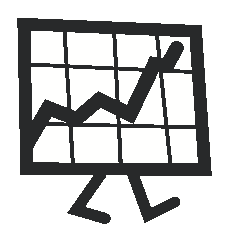
\includegraphics{justafigure}
\caption{Just a Figure\label{fig:justafigure}}
\end{figure}

\section{Figures and Tables}

Figures and tables must be referenced in the text by number.  They must be
numbered consecutively throughout each chapter, with the chapter number
preceding each figure or table number.  For example, the third figure in
chapter 1 would be labeled Figure 1.3.  You may either:
\begin{itemize}
\item Maintain one numbering sequence for figures and another for
  tables, and label figures with the word ``Figure'' and tables with the
  word ``Table''; or
\item Label both figures and tables with the word ``Figure'' and
  maintain one numbering sequence.
\end{itemize}
Place figures and tables as close to their references in the text as
possible.  Place a figure number and title below each figure (or table
labeled as a figure).  Place a table number and title above each table
labeled as a table.  In figures and tables, avoid using color and
avoid text smaller than 10 points.  Do not let figures or tables spill
out into the margins.  Figure~\ref{fig:justafigure} is an example figure.

\section{Lists}

You may include lettered, numbered, or bulleted lists in your thesis.
Use consistent punctuation and capitalization throughout each list.
Lists may be indented.

\section{Footnotes and Endnotes}

You may use footnotes or endnotes for brief notes that are not appropriate for
the body of the text.  Use either footnotes or endnotes consistently throughout
your thesis.  Position footnotes in 10 point type just above the bottom margin
and page number.  Use a short horizontal rule to separate footnotes from the
text.  Position endnotes at the end of each chapter.  Type endnotes using the
same font size and justification as the body of the text.  Single space within
each footnote or endnote; double-space between footnotes or endnotes.
Footnotes and endnotes should be consecutively numbered.

\section{Quotations}

You must use quotation marks and parenthetical references to indicate words
that are not your own. Put quotation marks around short quotes.  Put long
quotes in separate single-spaced paragraphs, indented up to 1 inch from the
left margin (these are called block quotations).  Kate Turabian, editor of
official publications and dissertation secretary at the University of Chicago
for over 25 years, distinguishes short and long quotes as follows:

\begin{quote}
  Short, direct prose quotations should be incorporated into the text
  of the paper and enclosed in double quotation marks: ``One small step
  for man; one giant leap for mankind.'' But in general a prose
  quotation of two or more sentences which at the same time runs to
  four or more lines of text in a paper should be set off from the
  text and indented in its entirety\dots~\cite{Turabian}
\end{quote}

\section{Equations}

Equations may be set in-line with the text or numbered and placed in separate
paragraphs.  Use the same numbering style for equations as you would for
figures and tables.  Here is an example of an equation set in-line with a
paragraph: $E = mc^2$.  Here is an example equation placed in a separate
paragraph:
\begin{equation}
E = mc^2
\end{equation}
Equation numbering and formatting should follow the usual convention of
your discipline and be acceptable to your thesis committee.

\newpage
\begin{table}[h]
	\caption{Thesis Formatting Options\label{tab:options}}
	\vspace{0.125in}
	\centering
	\hyphenpenalty10000  % turn off hyphenation in this table.  It looks bad.
	
	\begin{tabular*}{\textwidth}{|c|@{\extracolsep{\fill}}c|}
		\hline
		\textbf{Thesis Element} & \textbf{Formatting Options} \\ \hline
		\textbf{title page font} & \small 12-point or 14-point Garamond, Times or Roman \\ \hline
		\textbf{table of contents chapter title} & \small bold or plain \\
			\textbf{font} & \\ \hline
		\textbf{first-level table of contents} & \small 0 to 0.5 inch \\
			\textbf{indentation} & \\ \hline
		\textbf{second-level table of contents} & \small 0 to 1.0 inch \\
			\textbf{indentation} & \\ \hline
		\textbf{body text font} & \small 10, 11, or 12-point Garamond, Times or Roman \\ \hline
		\textbf{body text line spacing} & \small 1.5 or 2 \\ \hline
		\textbf{body text justification} & \small left or full \\ \hline
		\textbf{paragraph indentation} & \small 0 to 0.5 inch \\ \hline
		\textbf{chapter title position} & \small 1.5 to 3 inches below top edge of page \\ \hline
		\textbf{chapter title style} & \small heading preceded by the word ``Chapter'' and \\
			& \small the chapter number or, heading preceded only \\
			& \small by the chapter number \\ \hline
		\textbf{chapter title} & \small 10-pt to 36-pt font, centered or left-justified, \\
			& \small plain or bold \\ \hline
		\textbf{section heading} & \small 10-pt to 24-pt font, centered or left-justified, \\
			& \small plain or bold \\ \hline
		\textbf{subsection heading} & \small 10-pt to 18-pt font, centered or left-justified, \\
			& \small plain or bold \\ \hline
		\textbf{unnumbered headings} & \small 10-pt to 14-pt font, centered or left-justified, \\
			& \small plain or bold \\ \hline
		\textbf{table labels} & \small label tables as ``Table'' or ``Figure'' \\ \hline
		\textbf{Parenthetical reference style} & \small author-date system, numbered, or another style \\
			& \small acceptable to your committee \\ \hline
		\textbf{Reference list style} & any style acceptable to your committee \\ \hline
	\end{tabular*}
\end{table}

\fi

%%% Local Variables: 
%%% mode: latex
%%% TeX-master: "thesis-main"
%%% End: 
